\documentclass[11pt,twocolumn]{article}

\usepackage[margin=1in]{geometry}
\usepackage[T1]{fontenc}
\usepackage[utf8]{inputenc}
\usepackage{lmodern}
\usepackage{setspace}
\usepackage{graphicx}
\usepackage{subcaption}
\usepackage{hyperref}

\title{Examining the Pareto Frontier Between Model Size, Quantization Level, and Performance}
\author{Arthur L. Jackson \\ Johns Hopkins University}
\date{\today}

\begin{document}

\maketitle

\begin{abstract}
Large language models are increasingly con strained by deployment cost, making post training quantization an attractive way to re duce storage and hardware requirements without retraining. In this paper, we study the trade-offs between model size and performance with a Python quantization pipeline. We evaluate four pre-trained LLMs: Gemma 2 9B, Llama 3 8B, Mistral 7B, and Phi-3 Mini~\cite{gemma2,llama3herd,jiang2023mistral,abdin2024phi3}. We evaluate them under three manual weight-only quantization schemes: symmetric int8 per-tensor, symmetric int8 per-channel, and grouped symmetric int4. These quantized variants of the base LLM models are compared against their unquantized forms on two benchmarks; HellaSwag~\cite{zellers2019hellaswag} and MMLU~\cite{hendrycks2021mmlu}. We use normalized multiple choice scoring. 

The results show that int8 quantization typically preserves benchmark accuracy while substantially reducing artifact size, while grouped int4 yeilds the largest compression ratios but with the largest accuracy loss. In several model/quantizer pairs, quantized variants remain similar to raw baseline accuracy, suggesting that moderate post-training compression can be achieved with negligible degradation for some architectures. At the same time, the analysis reveals that quantization robustness is dependent on architecture. Per-channel scaling helps some models more than others, and aggressive int4 compression is markedly less stable on certain tasks. A secondary systems analysis shows that the storage frontier is real, but the runtime measurements in this pipeline are dominated by dense reconstruction of quantized models, rather than true low bit inference kernels. Overall, we provide both an empirical analysis and practical framework  for studying how quantization granularity ,compression ratio, and model family interact. 
\end{abstract}

\section{Introduction}
LLMs  have achieved strong performance across reasoning, text generation, and knowledge-intensive tasks. However, these gains come with substantial compute and storage costs. Even when a model has already been trained, deploying it remains expensive. Checkpoint files are large, memory requirements are high, and use is effectively limited to enterprise-grade hardware. Quantization is one of the most widely used strategies for reducing this deployment burden because it allows us to compress model weights into less precise vector representations while preserving performance~\cite{cheng2017compression,gholami2021surveyquantization,zhu2023llmcompression}. In practice, quantization is not a single design choice but an array of trade-offs involving precision level, scaling granularity, compression ratio, and model architecture.

In this paper, we study those tradeoffs through an evaluation of manual post training quantization. Rather than relying on a black-box quantization library, the project implements several weight-only quantization methods from scratch, and evaluates them under a common pipeline. This makes it possible to isolate how different quantization methods affect both model storage and benchmark accuracy, while also preserving the intermediate artifacts needed for deeper analysis. The central research question is as follows: how much performance can be retained as model size is reduced, and how does that relationship change across quantization schemes and model families?

To answer this question, the repository benchmarks four pretrained LLMs across raw, int8 per-tensor, int8 per-channel, and grouped int4 variants on HellaSwag~\cite{zellers2019hellaswag} and MMLU~\cite{hendrycks2021mmlu}. The goal is to map the Pareto frontier between compression and accuracy, but the resulting artifacts support a broader analysis as well. Because the pipeline records per-example prediction logs, confidence margins, artifact sizes, compression ratios, and systems-side measurements, it can also be used to study which quantization methods are more robust, where errors occur most frequently, and how reconstruction overhead affects evaluation. 

The contribution of this project contributes two things. First, it provides an empirical comparison of several hand-implemented weight only quantization methods across several model families and benchmarks, with attention to the tradeoff between storage savings and accuracy. Second, it contributes a reproducible evaluation framework for quantization research that captures both aggregate benchmark results and metadata needed for detailed analysis. The broader goal is to show that quantization can compress models and also characterize when that compression remains acceptable, when it fails, and which experimental changes matter most in making that distinction.

\section{Methodology}
We study post-training, weight only, quantization as a controlled intervention on a fixed set of pretrained LLMs. We implement a full pipeline end to end: downloading HuggingFace snapshots, quantizing selected model weights with manually-implemented low bit schemes, reconstructing quantized artifacts for evaluation, and benchmarking both raw and quantized variants on multiple choice reasoning tasks. The central experimental question is how much benchmark performance is lost as model storage is reduced, but the pipeline is designed so that every run also records timing, memory, and per-example prediction information as well as other metadata.

The evaluated models list consists of four enabled checkpoints in the project configuration. These are Gemma 2 9B, Llama 3 8B, Mistral 7B and Phi 3 Mini~\cite{gemma2,llama3herd,jiang2023mistral,abdin2024phi3}. For each model, we evaluate one unmodified raw baseline and three quantized variants, yielding a 32 run evaluation matrix across two benchmark tasks. The configuration file fixes the model revision, preferred floating point dtype, and whether remote model code should be trusted for loading. Models are first downloaded to a local raw snapshot directory and all subsequent quantization and evaluation steps operate on those local copies rather than fetching weights during benchmarking. This design reduces run to run variation caused by remote updates and makes the experiment reproducible from a single configuration file.

Quantization is applied only to tensors corresponding to ‘torch.nn.Linear’ weights. The repository identifies these tensors by instantiating the model structure with empty weights and collecting the parameter names of all linear modules. All other tensors, such as embed dings, normalization parameters, and other non linear weights, are passed through to the arti fact without low bit compression. This choice isolates the effect of compressing the domi nant matrix-multiplication weights while avoiding architecture-specific modifications to the rest of the checkpoint. Quantized artifacts are written as shared ‘safetensors’ files together with a .JSON manifest that records tensor level metadata, original shapes and dtypes, quantization parameters, and size statistics. 

The first quantization family is symmetric int8 quantization~\cite{wu2020integerquantization,dettmers2022llmint8,xiao2023smoothquant}. For per tensor int8, each linear weight matrix $W$ is assigned a single scale $s = \max(|W|)/127$, and every element is quantized by rounding $W/s$ to the nearest integer and clipping to the signed int8 range $[-127,127]$. For per-channel int8, the same symmetric rule is applied independently along channel axis 0, which corresponds to output rows for linear layers in this implementation. Per-channel scaling increases metadata overhead because one scale must be stored for each output channel, but it better preserves weights whose dynamic ranges differ substantially across rows.

The second family is grouped symmetric int4 quantization. Each linear weight tensor is reshaped into a two dimensional matrix, partitioned row-wise into fixed groups of 128 values, and assigned one scale per group using $s_g = \max(|W_g|)/7$. Values are then rounded and clipped into the signed int4 range $[-7,7]$. To reduce storage further, two 4-bit values are packed into a single byte after shifting the signed range by a storage zero-point of 8. Groupwise scaling provides a compromise between global scaling, which is compact but inaccurate, and fully local scaling, which is accurate but expensive to store. Because the implementation is manual and educational rather than kernel optimized, the artifact stores packed weights and scales for later reconstruction rather than using a custom low-bit inference kernel directly.

Evaluation is performed on HellaSwag~\cite{zellers2019hellaswag} and MMLU~\cite{hendrycks2021mmlu} using the Hugging Face \texttt{datasets} interface. HellaSwag is evaluated on the validation split and MMLU is evaluated on the \texttt{all} configuration of the test split. Prompts are rendered in plain text by default even when a tokenizer exposes a chat template. This is an important experimental control: chat templates differ across model families and can otherwise change likelihood scoring independently of quantization. Each example is wrapped in a fixed system instruction and user prompt. HellaSwag examples present a scenario context and the model must score four candidate endings. MMLU examples present a question and four answer choices. Instead of scoring only the bare labels \texttt{A}, \texttt{B}, \texttt{C}, and \texttt{D}, the implementation scores full answer continuations of the form ``A. <choice>'' in order to reduce label-position bias in base language models.

For both benchmarks, prediction is based on normalized continuation log likelihood. Let $x$ denote the rendered prompt and $y_i$ a candidate continuation. The model computes the token log probability of the full sequence $x \Vert y_i$, and the score for candidate $i$ is the sum of log probabilities over the continuation tokens divided by the number of continuation tokens. Normalizing by continuation length is necessary because HellaSwag endings and MMLU answers are not all tokenized to the same length. The predicted answer is the candidate with the highest normalized score. This scoring rule is applied identically to raw and quantized variants so that any performance differences arise from the quantized weights rather than from different prompting or decoding settings.

Quantized models are evaluated by reconstructing a standard dense Transformers model from the saved artifact. The loader reads the manifest, restores pass-through tensors directly, dequantizes int8 or int4 weight tensors back to their original floating-point dtype, and loads the resulting state dictionary into an \texttt{AutoModelForCausalLM} instance. This design is important for interpretation. It means that reported benchmark accuracy is a valid measure of information loss due to quantization, and reported disk size is a valid measure of storage savings, but runtime measurements should not be interpreted as the performance of a production low-bit serving stack. Since inference is executed on reconstructed dense tensors rather than specialized low bit kernels, the benchmarks measure model quality under quantization and the cost of reconstruction-based evaluation, not the full systems benefit of optimized int4/int8 deployment.

To support reproducibility and downstream analysis, every benchmark run writes both a summary .json file and a per-example .jsonl file. The summary includes accuracy, correct count, example count, model load time, evaluation time, examples per second, average prompt length, average predicted continuation length, total forward passes, and peak CUDA memory usage when a GPU is available. For quantized variants, the summary also includes original artifact size, quantized artifact size, quantization runtime, and the resulting compression ratio. The per-example records preserve the example identifier, benchmark metadata such as MMLU subject or HellaSwag split type, the score assigned to each answer option, the predicted label, correctness, and the score margin between the top two candidates. Taken together, these artifacts make it possible to reproduce the headline Pareto analysis while also enabling finer grained studies of where and why quantization changes model behavior.

\section{Experiments}
The experimental setup is organized around direct comparisons between each raw model and its three quantized counterparts. For every model, the raw checkpoint serves as the baseline and is evaluated alongside int8 per channel, int8 per tensor, and grouped int4 variants under the same prompting and scoring protocol. No calibration set, quantization aware fine-tuning or post quantization retraining is used. This keeps our study focused on post training, weight only compression and makes the differences attributable to the quantization method itself instead of to additional adaption stages. The full evaluation matrix therefore consists of four model families, four variants of each model, and two benchmarking tests. This gives us a total of 32 benchmark summaries.

We report two classes of evaluation metrics. The primary task quality metric is multiple choice accuracy based on HellaSwag and MMLU. For each benchmark run, we also store the number of correct preidctions, evaluated samples, per example choice scores, and the margin between the top two normalized log-likelihoods. These fields make accuracy the most important metric while preserving enough information for other error analysis. The primary compression metrics are quantized artifact size (bytes), absolute storage saved relative to original raw model, and compression ratio. Together, these metrics define the size/performance Pareto frontier that motivates this research paper.

In addition to these metrics, we evaluate several secondary systems oriented measurements. Each benchmark summary records model load time, evaluation time, examples processed (per second) and peak CUDA memory usage. Since the current pipeline reconstructs quantized models back into their dense model forms before performing inference, these measurements are interpreted as artifact reconstruction and dense evaluation costs rather than as production low bit serving efficiency. However, this is still useful because we can compare the practical overhead introduced by different quantization schemes within our own evaluation framework. 

The analysis is structured around three comparisons. First, we perform a compression efficiency analysis that asks how much accuracy is retained for each unit of storage reduction. In practice, this means comparing raw and quantized accuracy against both absolute gigabyte storage saved and compression ratio. This allows us to identify which quantizers produce the strongest quality/size tradeoff for each architecture. Second, we study systems-side tradeoffs by comparing load time, evaluation time, throughput, and peak memory across variants. This analysis is not used to claim true low bit runtime gains, but rather to show how different artifact formats affect the cost of reconstruction based evaluation. Third, we conduct a scheme-level robustness analysis focused on int8 per channel vs. int8 per tensor scaling. This isolates whether finer quantization granularity improves benchmark preservation consistently, or whether its benefit depends on model family and task.

The benchmark artifacts also enabled several sensitivity analysis even without changing the core pipeline. Since the saved predictions include benchmark specific metadata such as HellaSwag split type and MMLU subject, quantization effects can be examined at the level of domain area, subject area, or confidence margin rather than only total accuracy. These analyses are treated as secondary to the main frontier study but they provide and important check on whether quantization degrades all tests uniformly or affects certain parts disproportionately. The experiments are designed not only to rank quantization schemes, but also to characterize how and where performance changes occur.  

\section{Results}
The benchmark results show a consistent overall pattern: moderate weight-only quantization often preserves model quality surprisingly well, but more aggressive compression produces less stable outcomes. Across both HellaSwag and MMLU, the int8 variants generally remain close to the raw baselines while reducing artifact size substantially, whereas grouped int4 achieves the largest storage reductions with a wider spread in retained accuracy. This pattern is visible in the compression-efficiency plots in Figure~\ref{fig:compression-efficiency}, where most int8 points remain clustered near the raw-accuracy line while int4 points extend farther along the storage axis with more variable vertical placement.

Compression-efficiency analysis confirms that int8 quantization usually provides the strongest quality-size tradeoff. On HellaSwag, Phi-3 with int8 per-channel retains 101.72\% of raw accuracy while saving 3.46 GB, and Gemma-2 9B with int8 per-tensor retains 99.84\% of raw accuracy while saving 23.26 GB. On MMLU, Gemma-2 9B with int8 per-tensor reaches 112.49\% of the raw baseline while saving 23.26 GB, and Phi-3 with int8 per-channel retains 100.91\% while saving 3.46 GB. These cases should not be interpreted as evidence that quantization systematically improves models; rather, they indicate that for some model-task pairs, the measured degradation is small enough to fall within the variability of the evaluation setup. By contrast, the most aggressive compression point---Gemma-2 9B with grouped int4---saves 26.89 GB at a compression ratio of 4.57$\times$, but its MMLU retention falls to 62.96\%, illustrating that larger storage gains can come with meaningful quality loss.

The results also show that quantization sensitivity is architecture-dependent rather than uniform across the model suite. Llama-3 8B and Phi-3 are comparatively robust under several quantized settings, with some variants matching or slightly exceeding the raw baselines on individual benchmarks. Mistral-7B is similarly stable under int8 but shows a clearer drop under grouped int4 on HellaSwag. Gemma-2 9B exhibits the widest spread between favorable and unfavorable settings: its int8 variants remain competitive, but grouped int4 produces the most severe benchmark degradation observed in the study. Taken together, these results suggest that the Pareto frontier is not defined only by bit-width; it is also shaped by how a given model family responds to quantization granularity.

\begin{figure*}[t]
\centering
\begin{subfigure}{0.48\textwidth}
\centering
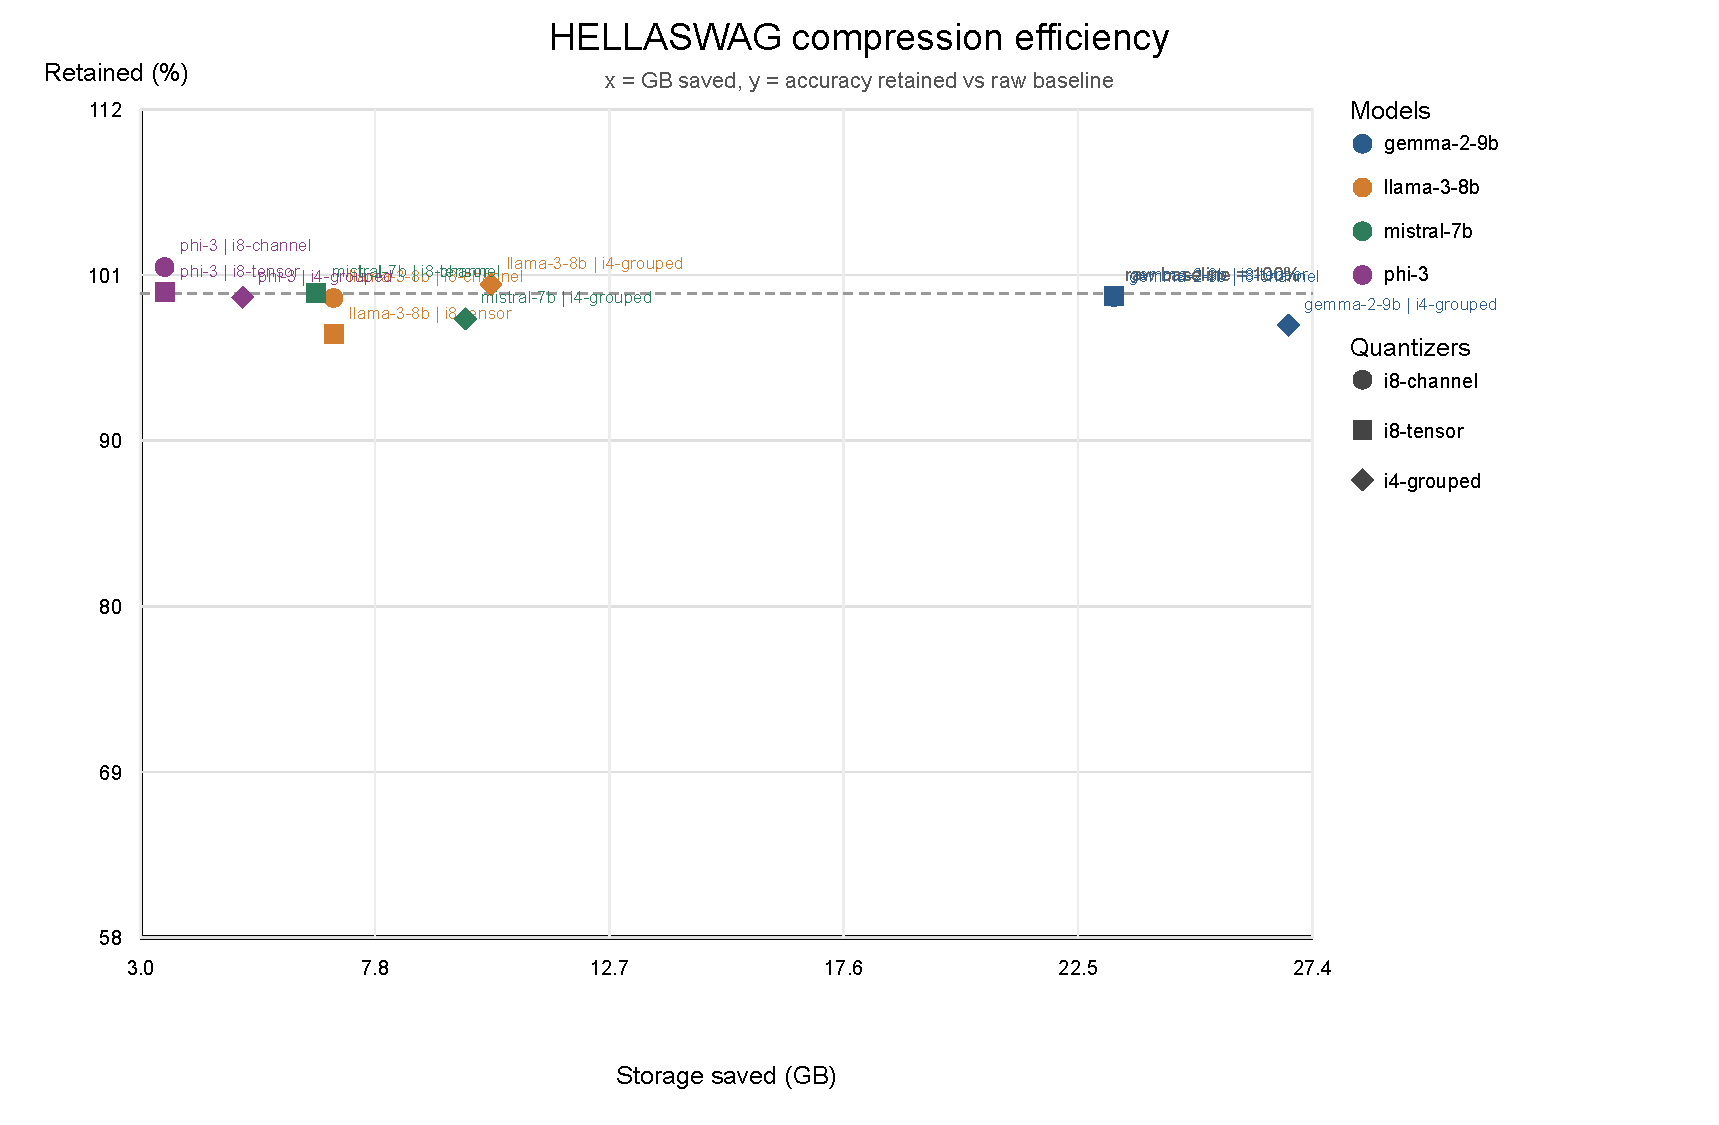
\includegraphics[width=\linewidth]{../analysis/compression_efficiency_hellaswag.pdf}
\caption{HellaSwag compression efficiency.}
\end{subfigure}
\hfill
\begin{subfigure}{0.48\textwidth}
\centering
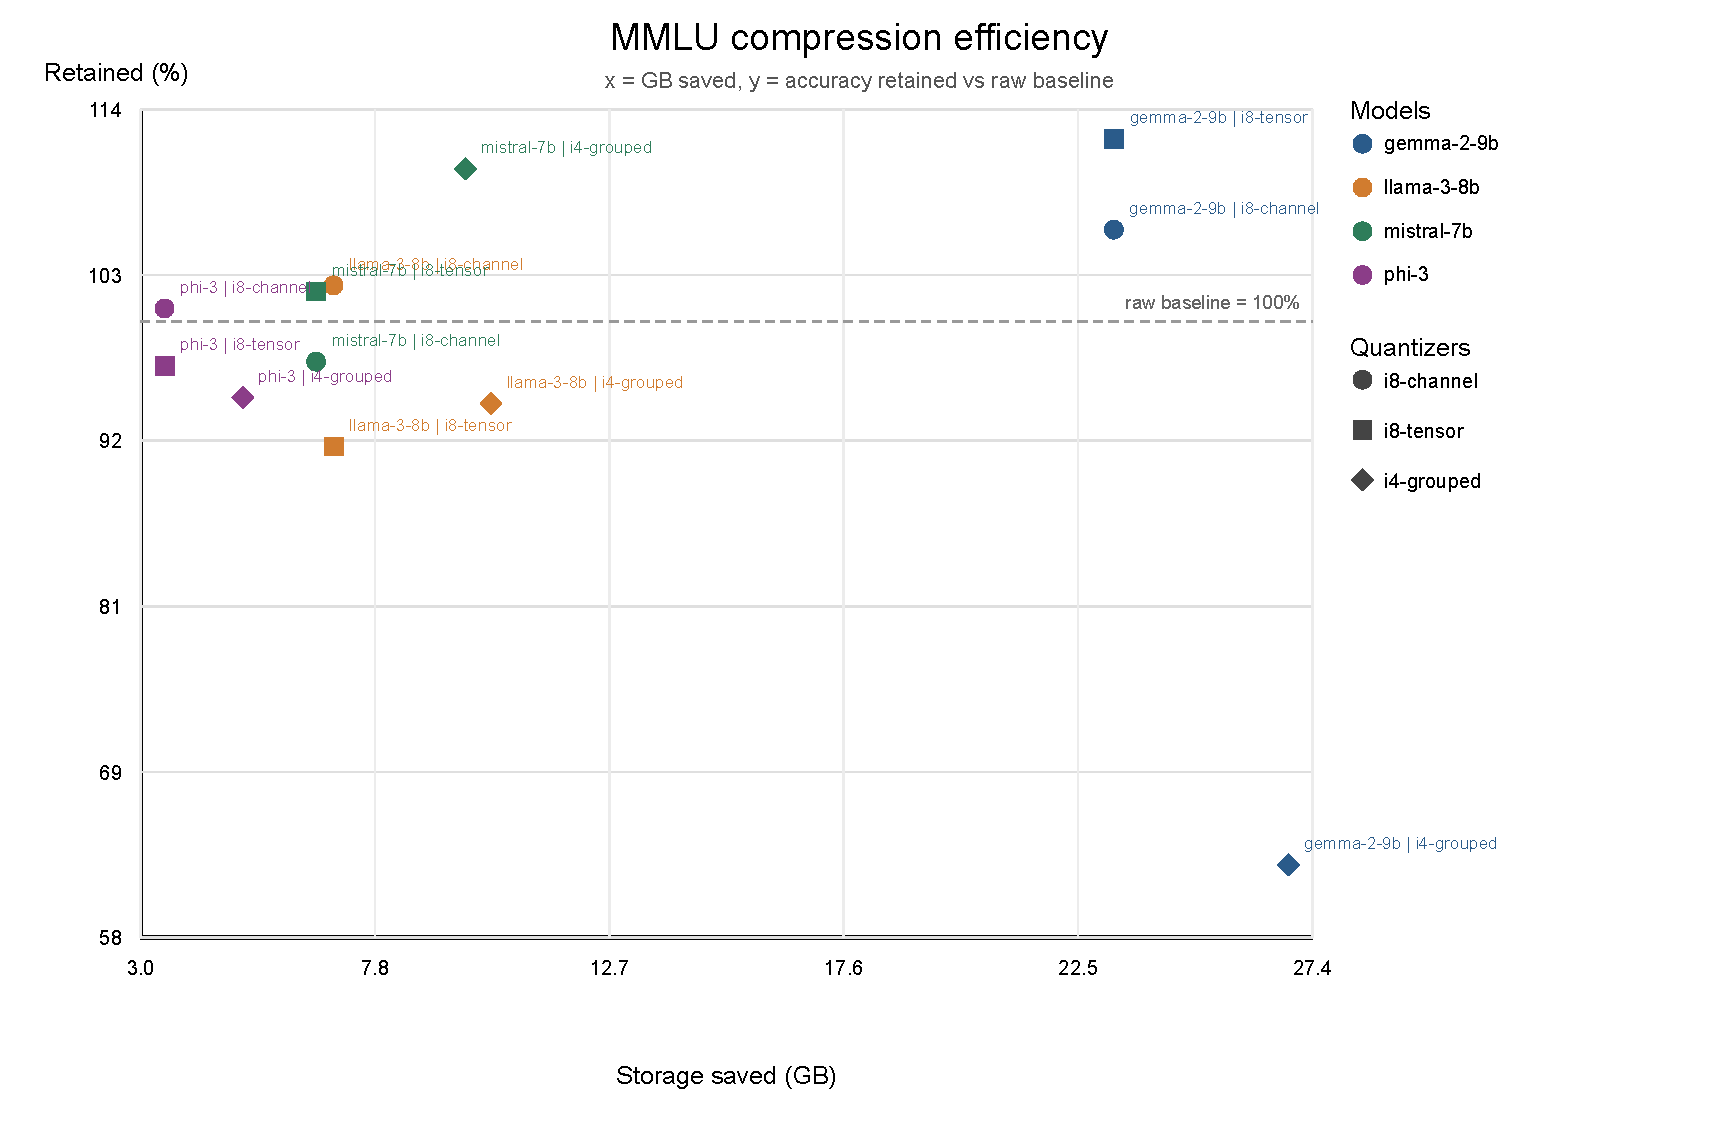
\includegraphics[width=\linewidth]{../analysis/compression_efficiency_mmlu.pdf}
\caption{MMLU compression efficiency.}
\end{subfigure}
\caption{Compression-efficiency analysis for the two benchmark tasks. Points farther to the right save more storage; points higher on the plot retain more of the raw model's accuracy.}
\label{fig:compression-efficiency}
\end{figure*}

Scheme-level robustness analysis further clarifies that the benefit of finer scaling granularity is real but not universal. Figure~\ref{fig:int8-robustness} plots the accuracy difference between int8 per-channel and int8 per-tensor quantization for each model family. On HellaSwag, the mean channel-minus-tensor advantage is +0.0069, with the clearest gains appearing for Llama-3 8B (+0.0163) and Phi-3 (+0.0120), while Gemma-2 9B is nearly tied and Mistral-7B is exactly tied. On MMLU, the average advantage is smaller at +0.0041 and the model-specific differences are mixed: per-channel scaling helps Llama-3 8B (+0.0328) and Phi-3 (+0.0267), but per-tensor scaling is stronger for Gemma-2 9B (-0.0273) and Mistral-7B (-0.0158). The implication is that per-channel quantization should be treated as a useful but architecture-sensitive refinement rather than as a universally dominant choice.

The systems-side results, summarized in Figure~\ref{fig:systems-tradeoffs}, are informative but require careful interpretation. The generated summaries show large load-time penalties for quantized artifacts relative to the raw baselines, especially for grouped int4, and they show that throughput is often comparable to raw inference for some models but substantially worse for others. These measurements do not indicate that low-bit inference is intrinsically slower; instead, they reflect the repository's evaluation design, which reconstructs a dense model from the quantized artifact before benchmarking. Within that constraint, the systems plots still reveal meaningful differences in reconstruction overhead. In particular, grouped int4 consistently incurs the largest loading cost because its packed representation must be explicitly unpacked and dequantized before evaluation, while the int8 variants are less expensive to reconstruct. Peak CUDA memory is largely unchanged for most models, but Gemma-2 9B shows roughly a twofold increase in peak allocation for quantized variants under the current pipeline.

\begin{figure*}[t]
\centering
\begin{subfigure}{0.48\textwidth}
\centering
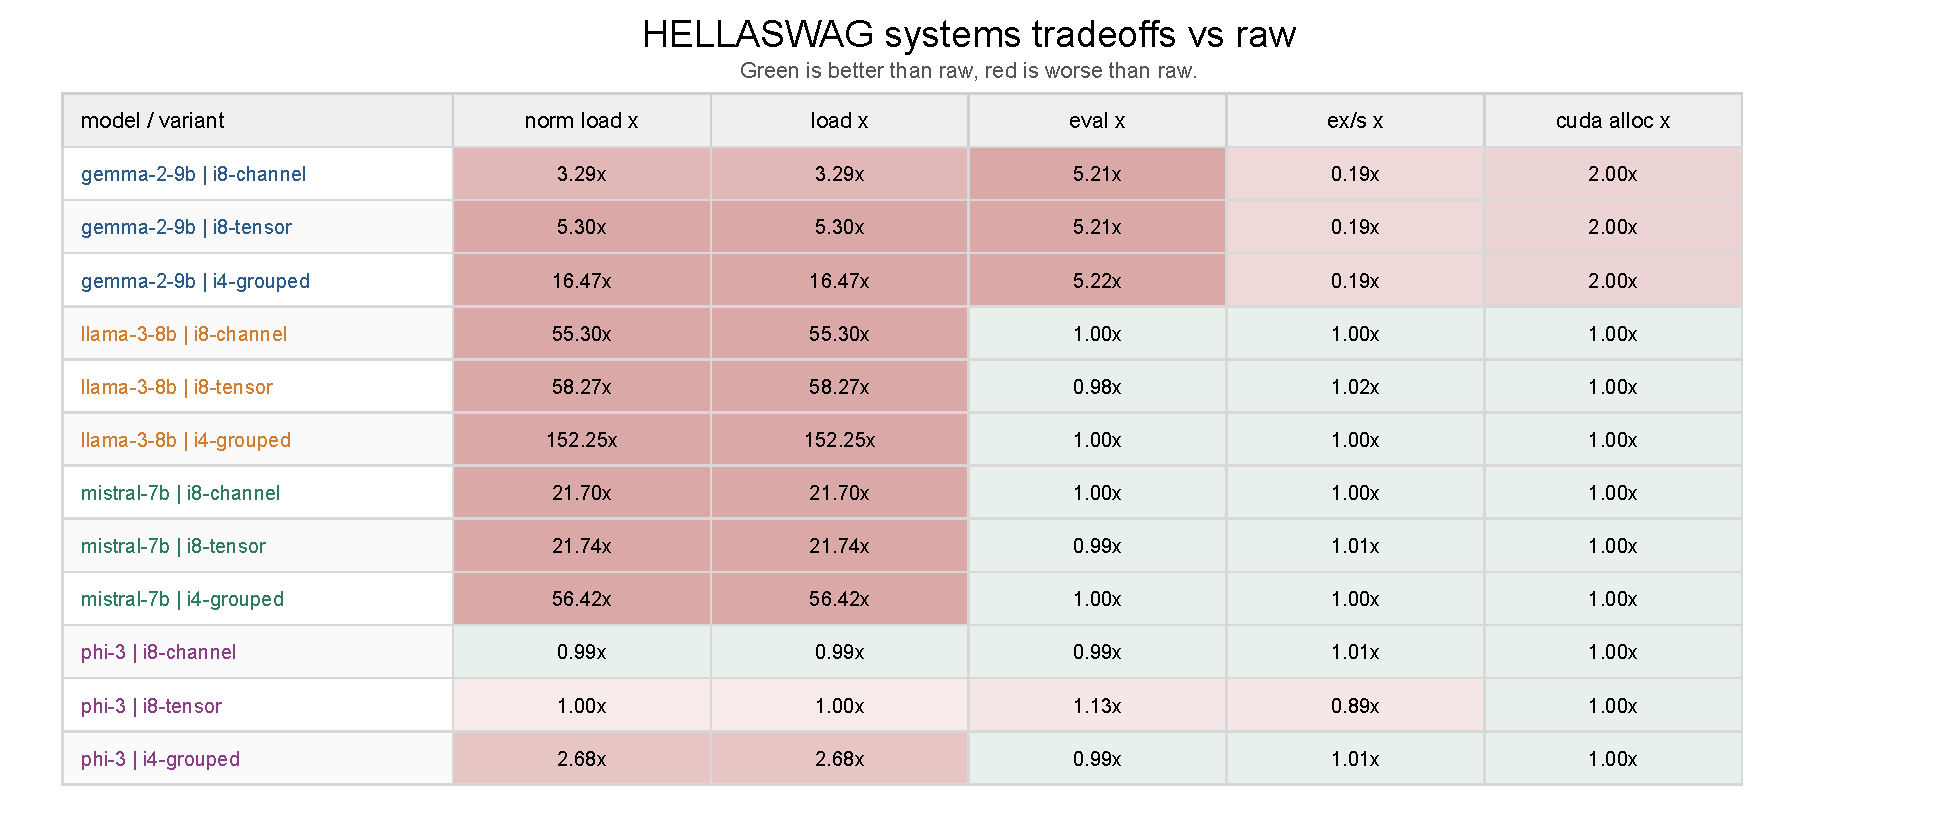
\includegraphics[width=\linewidth]{../analysis/systems_tradeoffs_hellaswag.pdf}
\caption{HellaSwag systems tradeoffs.}
\end{subfigure}
\hfill
\begin{subfigure}{0.48\textwidth}
\centering
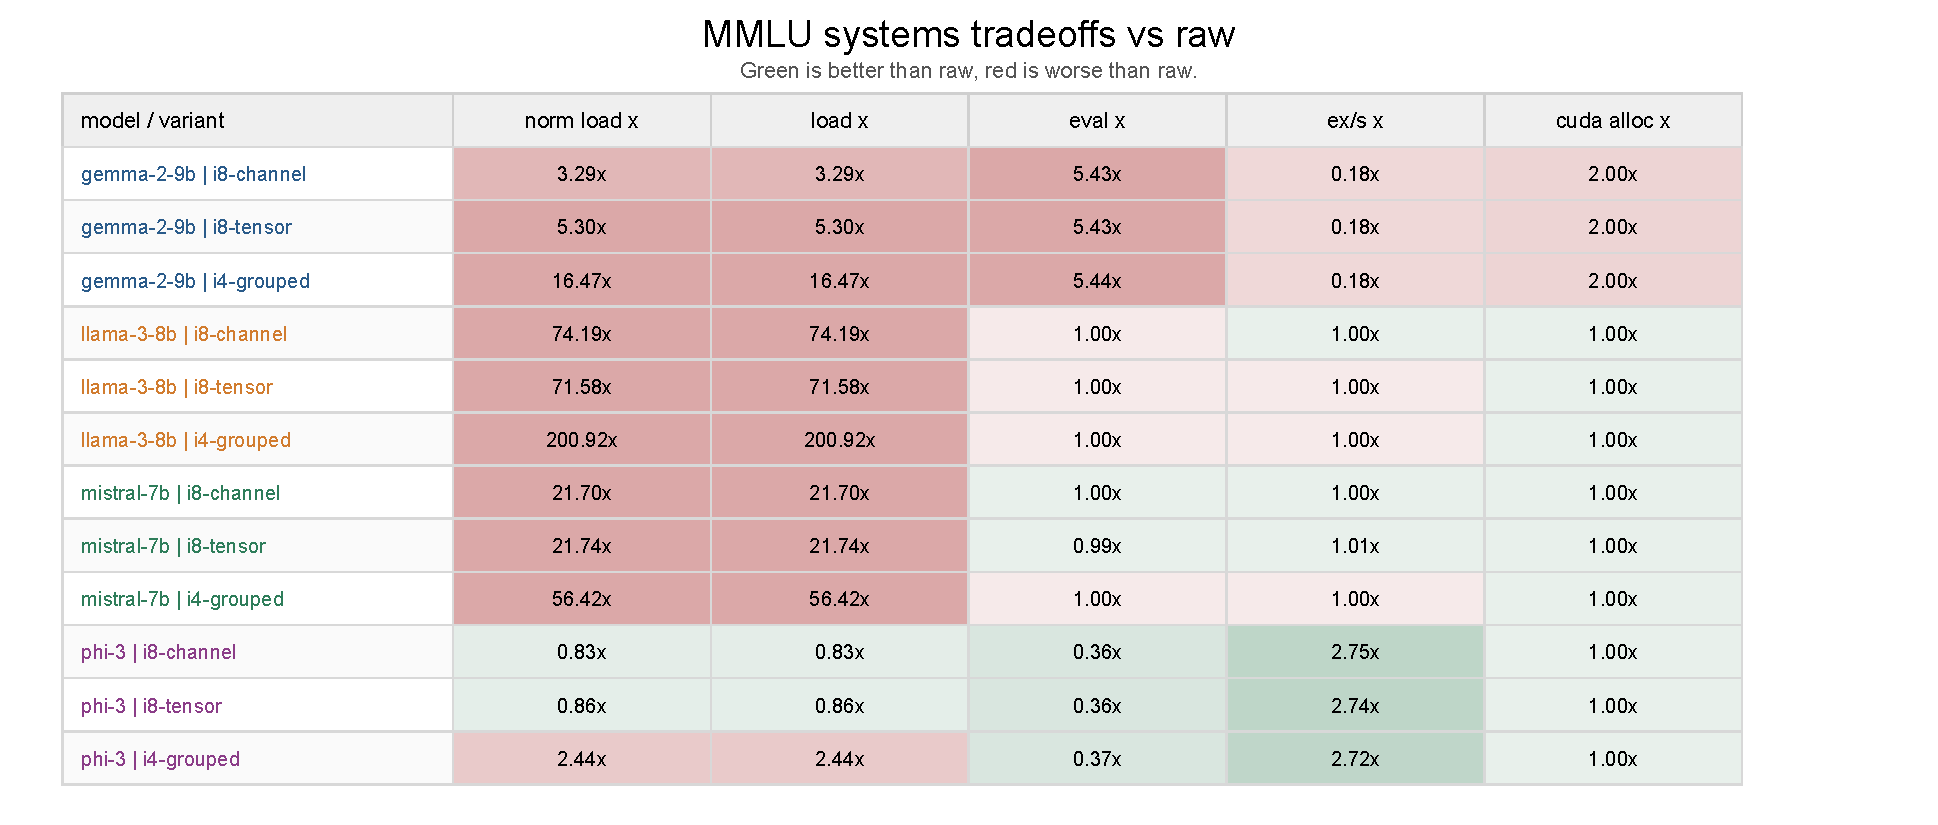
\includegraphics[width=\linewidth]{../analysis/systems_tradeoffs_mmlu.pdf}
\caption{MMLU systems tradeoffs.}
\end{subfigure}
\caption{Systems-oriented measurements relative to each raw baseline. These values reflect reconstruction-based evaluation overhead rather than production low-bit serving speed.}
\label{fig:systems-tradeoffs}
\end{figure*}

\begin{figure}[t]
\centering
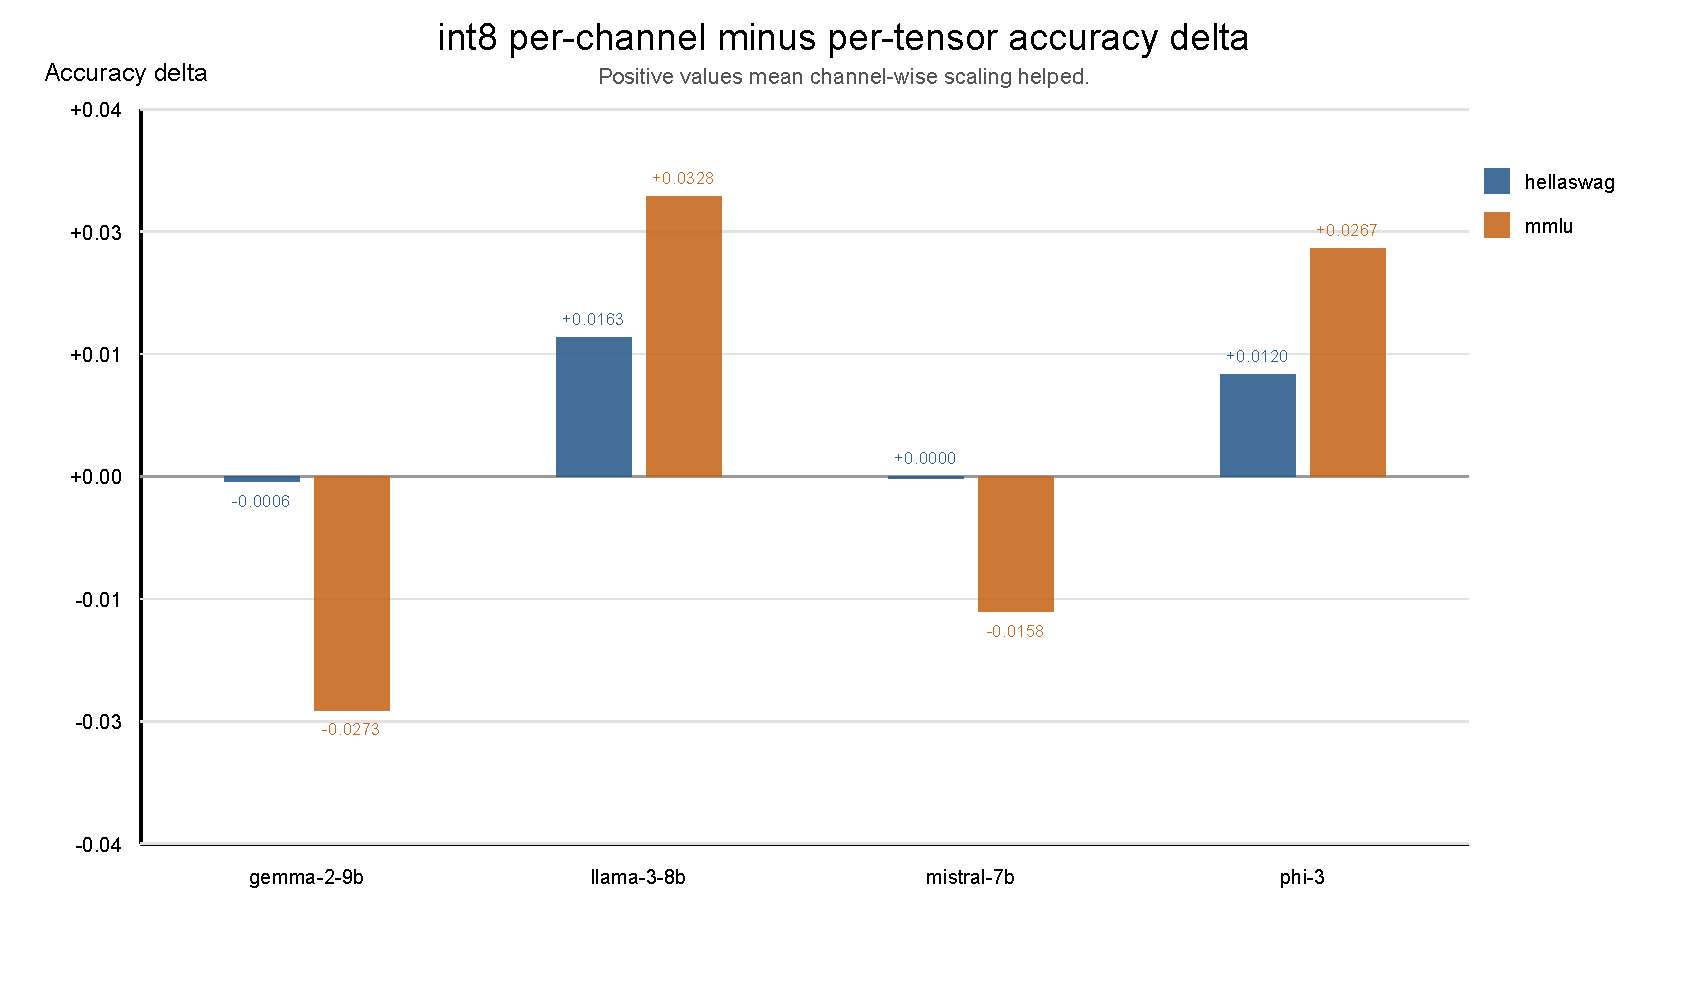
\includegraphics[width=\columnwidth]{../analysis/int8_channel_vs_tensor.pdf}
\caption{Accuracy delta between int8 per-channel and int8 per-tensor quantization. Positive values indicate that per-channel scaling performed better.}
\label{fig:int8-robustness}
\end{figure}

Overall, the results support three main conclusions. First, the empirical Pareto frontier is real: substantial storage savings are achievable with modest or inconsistent accuracy loss, especially under int8 quantization. Second, grouped int4 provides the strongest compression but is the least predictable setting in terms of downstream quality. Third, the effect of quantization granularity depends on the model family, so architecture-aware comparisons are necessary when selecting a compression scheme. These findings motivate the later discussion of why aggregate benchmark averages are useful but insufficient on their own for understanding quantization behavior.

\section{Discussion}
The results suggest that the most practically useful region of the studied frontier lies in moderate weight-only compression rather than in the most aggressive low-bit setting. Across the evaluated models, symmetric int8 quantization usually preserves benchmark accuracy closely while still delivering meaningful storage savings. This makes int8 the strongest default choice in the current pipeline when the goal is to reduce artifact size without materially changing downstream behavior. Grouped int4, by contrast, moves farther along the compression axis but introduces substantially more variance in retained accuracy. In other words, the frontier is favorable, but it is not flat: larger compression gains are achievable, yet they come with a more fragile quality profile.

The pattern is also informative at the architectural level. Per-channel int8 often helps relative to per-tensor scaling, but not uniformly. A plausible explanation is that some models contain larger row-to-row variation in linear-layer weight magnitudes, making local scaling more useful, whereas other architectures are already well served by a single tensor-wide scale. The grouped int4 results point to the opposite side of this tradeoff. Reducing precision to four bits yields a much coarser representation, so even with group-wise scaling the quantizer has less capacity to preserve subtle weight differences. The strongest implication is therefore not simply that ``lower bit-width is worse,'' but that quantization behavior depends on the interaction between bit-width, scaling granularity, and model family.

At the same time, the study has important limitations that constrain how broadly the results should be interpreted. First, the benchmark suite is narrow: HellaSwag and MMLU are useful multiple-choice evaluations, but they do not cover generation quality, calibration, long-context behavior, or instruction-following performance. Second, the analysis is limited to a small set of manually implemented weight-only quantizers and does not include activation quantization, mixed precision, calibration-based post-training methods, or quantization-aware finetuning. Third, only \texttt{torch.nn.Linear} weights are quantized, while embeddings, normalization parameters, and other tensors are preserved in higher precision. The results therefore isolate a meaningful and common compression target, but they do not represent full-model quantization in the broadest sense.

The systems measurements require especially careful interpretation. Because quantized artifacts are reconstructed into dense floating-point models before inference, the reported load time, throughput, and memory values are not estimates of a production low-bit serving stack. They instead measure the overhead of this repository's reconstruction-based evaluation path. This is still useful for understanding the engineering cost of the current pipeline, but it means the paper should not claim that int4 or int8 inference is inherently slower than raw inference. A related limitation is that small accuracy gains over raw baselines should not be treated as genuine improvements in model capability. In this setting, they are better interpreted as evidence that some quantized variants remain close enough to the raw model that the observed differences are small relative to the granularity of the benchmark outcome.

These limitations also point directly to future work. The most important extension would be to pair the current artifact-level analysis with true low-bit inference backends so that storage, latency, throughput, and memory could be evaluated under a deployment-realistic kernel implementation rather than dense reconstruction. Additional work should broaden the benchmark set, pin exact model and dataset revisions for stronger long-term reproducibility, and test richer quantization families such as mixed-precision or layer-wise schemes. Finally, the saved per-example predictions make it possible to go beyond aggregate accuracy by studying failure concentration across MMLU subjects, HellaSwag split types, and confidence margins. That type of analysis would strengthen the central contribution of the project: not only identifying where the Pareto frontier lies, but also explaining where quantization changes model behavior and where it remains surprisingly robust.

\section{Conclusion}
This paper examined the tradeoff between model compression and downstream performance through a reproducible, from-scratch post-training quantization pipeline for causal language models. Across four model families and two multiple-choice benchmarks, the results showed that weight-only int8 quantization generally offers the strongest balance between storage savings and accuracy retention, while grouped int4 provides larger compression gains at the cost of less stable task performance. The study also found that quantization behavior is architecture-dependent: per-channel scaling improves robustness for some models, but its benefit is not universal across tasks or model families.

Beyond the Pareto frontier itself, the project contributes an evaluation framework that preserves artifact metadata, per-example predictions, confidence margins, and system-side measurements for deeper analysis. These outputs make it possible to move beyond headline accuracy and study when quantization changes model behavior, which schemes are more robust, and how compression interacts with benchmark difficulty and model architecture. At the same time, the experiments clarify an important methodological boundary: because quantized artifacts are reconstructed into dense models before evaluation, the measured runtime characteristics should be interpreted as reconstruction overhead rather than as true low-bit serving efficiency. Future work should pair the current accuracy-focused framework with production-style low-bit inference kernels, broader benchmark coverage, and layer-wise or mixed-precision quantization strategies to better understand how practical deployment constraints interact with model quality.

\bibliographystyle{plain}
\bibliography{references}

\end{document}
